
In each of these three simulations, all of the components were represented 
by the Lumped Parameter model.  The transit time was selected to be equal to one time step for each component. For the buffer component, the porosity was selected to be zero to halt flow.


In the first of these simulations, the Piston Flow Model (PFM) was 
selected from among the three response functions. 
\begin{figure}[ht!]
\centering
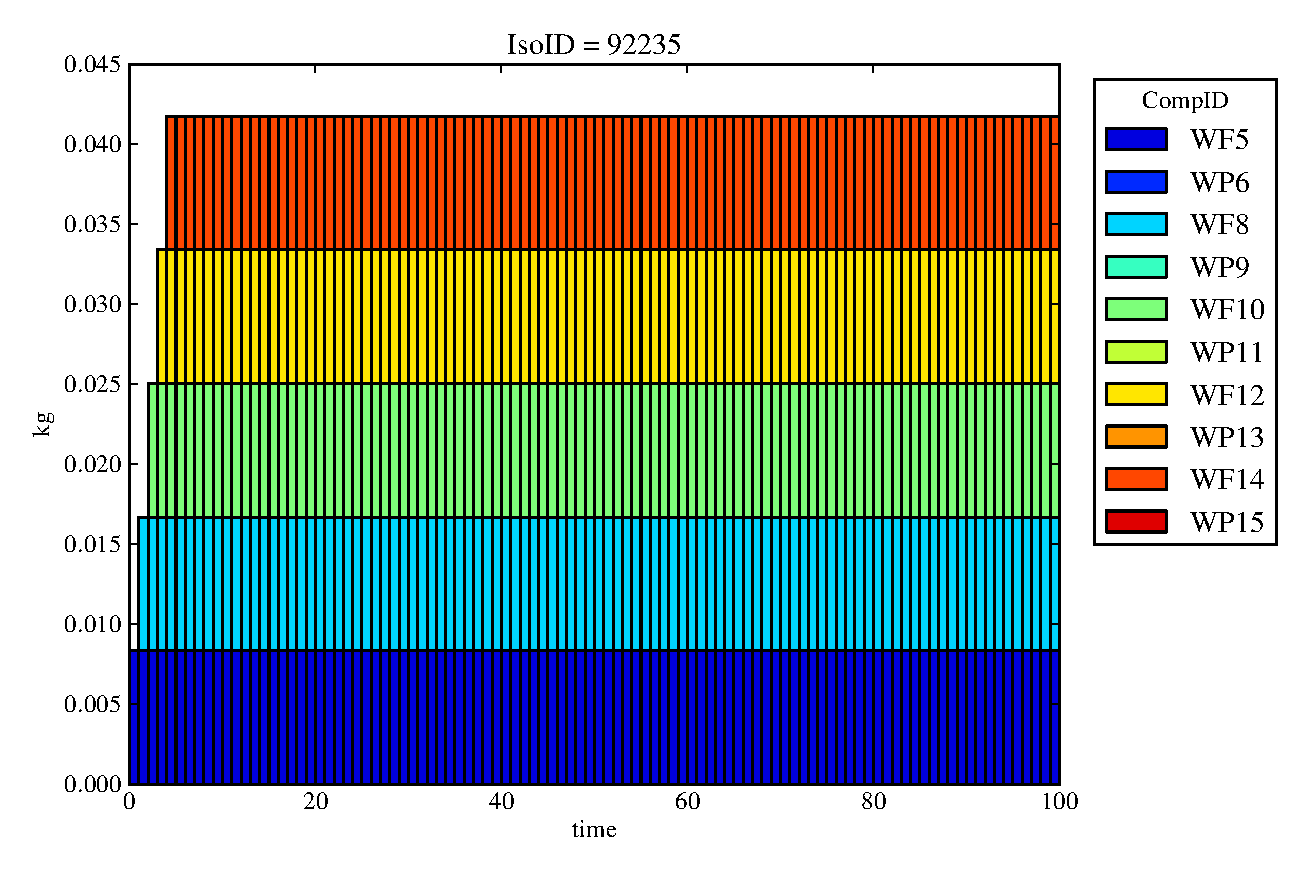
\includegraphics[width=0.6\textwidth]{./chapters/demonstration/base/lpPFMII.eps}
\caption[$^{235}U$ residence. Lumped Parameter PFM Waste Package No Release.]{
For case LPPFMII in which total containment in the waste package is assumed 
($F_{d,wp}=0$), $^{235}U$ travels through the waste form component ($F_d = 0.1$) before 
permanent residence in the waste package component.
}
\label{fig:lpPFMIIall}
\begin{minipage}[b]{0.45\linewidth}
  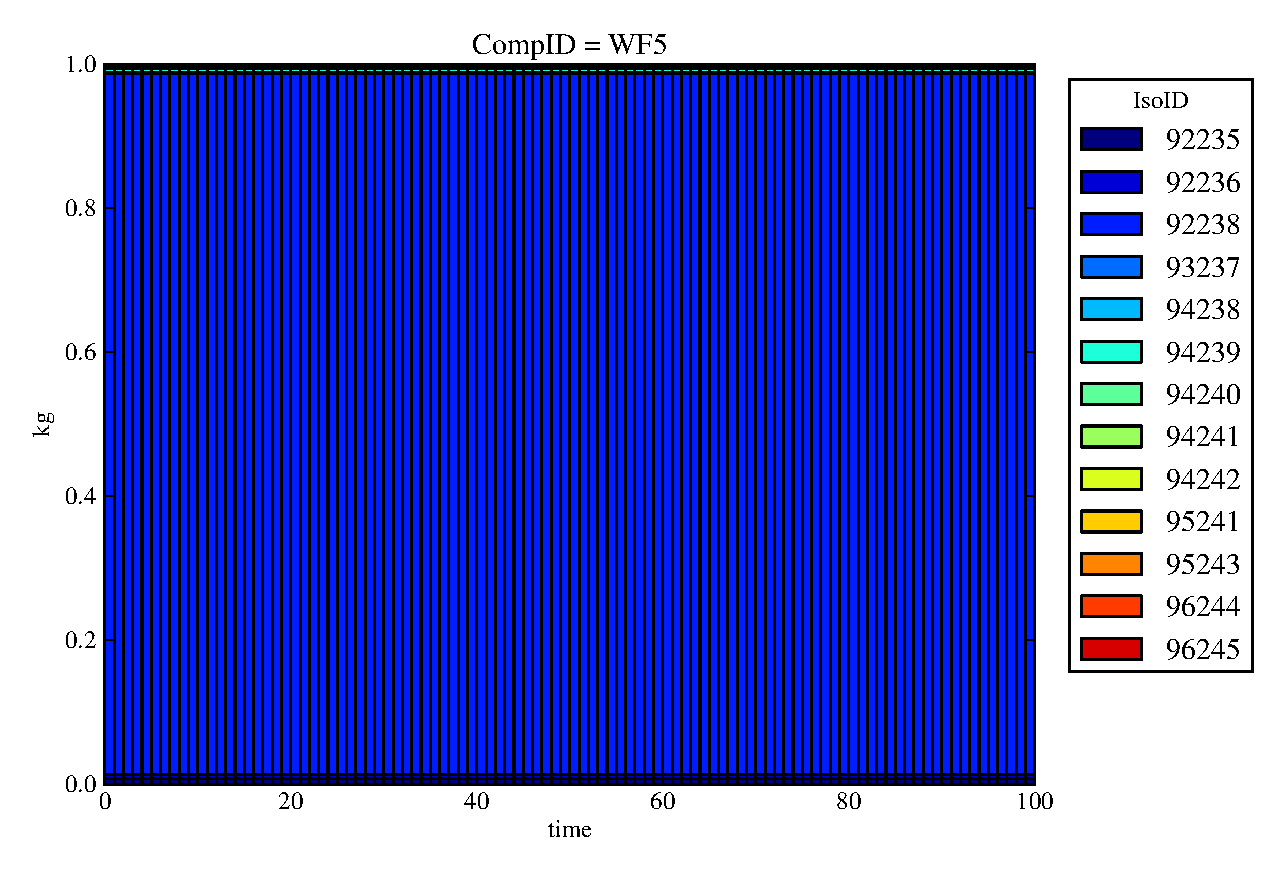
\includegraphics[width=\textwidth]{./chapters/demonstration/base/lpPFMII1.eps}
  \caption[Case LPPFMII Waste Form Contaminants.]{
    Waste Form 5 ($F_d = 0.1$) releases material with degradation. 
    }
  \label{fig:lpPFMIIwf5}
  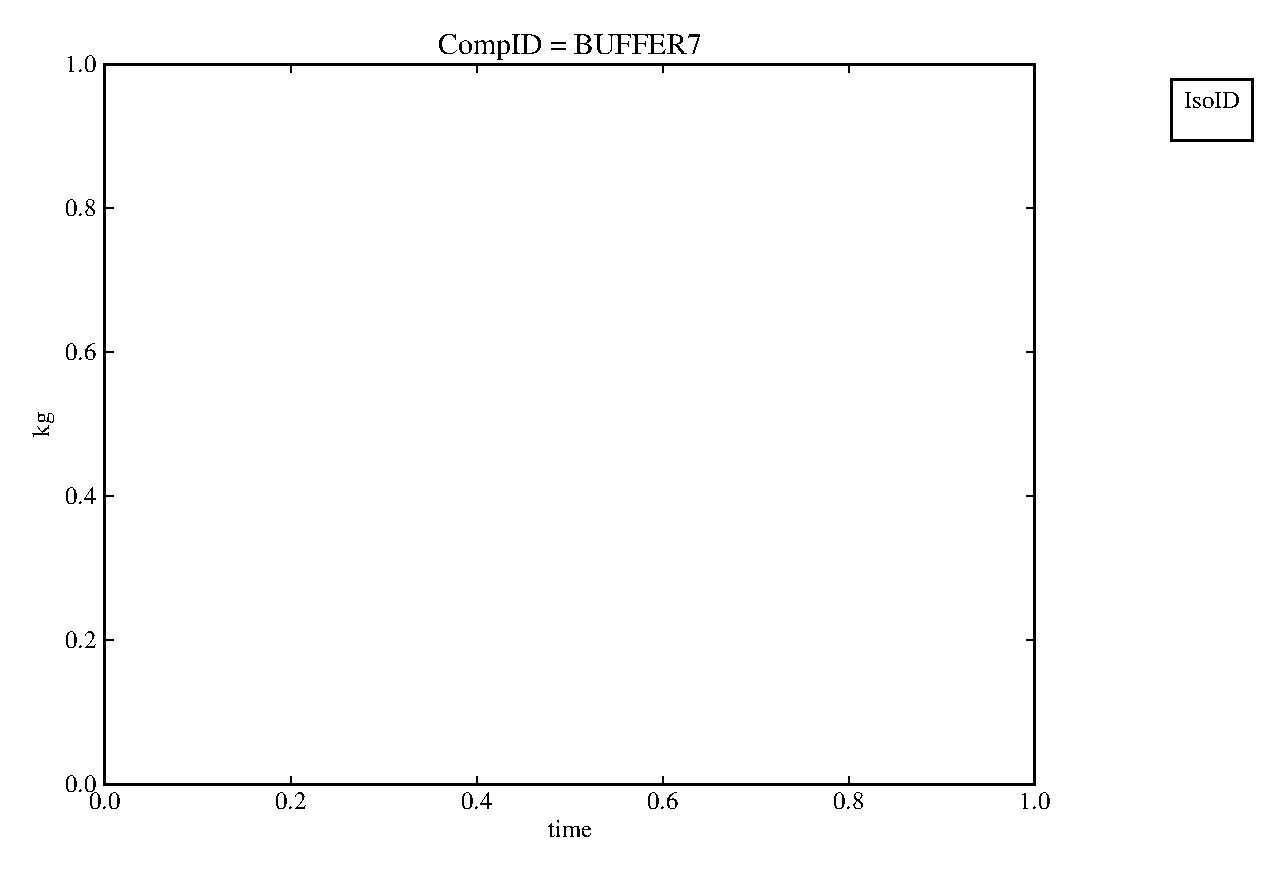
\includegraphics[width=\textwidth]{./chapters/demonstration/base/lpPFMII3.eps}
  \caption[Case LPPFMII Buffer Contaminants]{
    The Buffer, component 7 ($F_d=0$), never receives material.
    }
  \label{fig:lpPFMIIbuff}

\end{minipage}
\hspace{0.05\linewidth}
\begin{minipage}[b]{0.45\linewidth}
  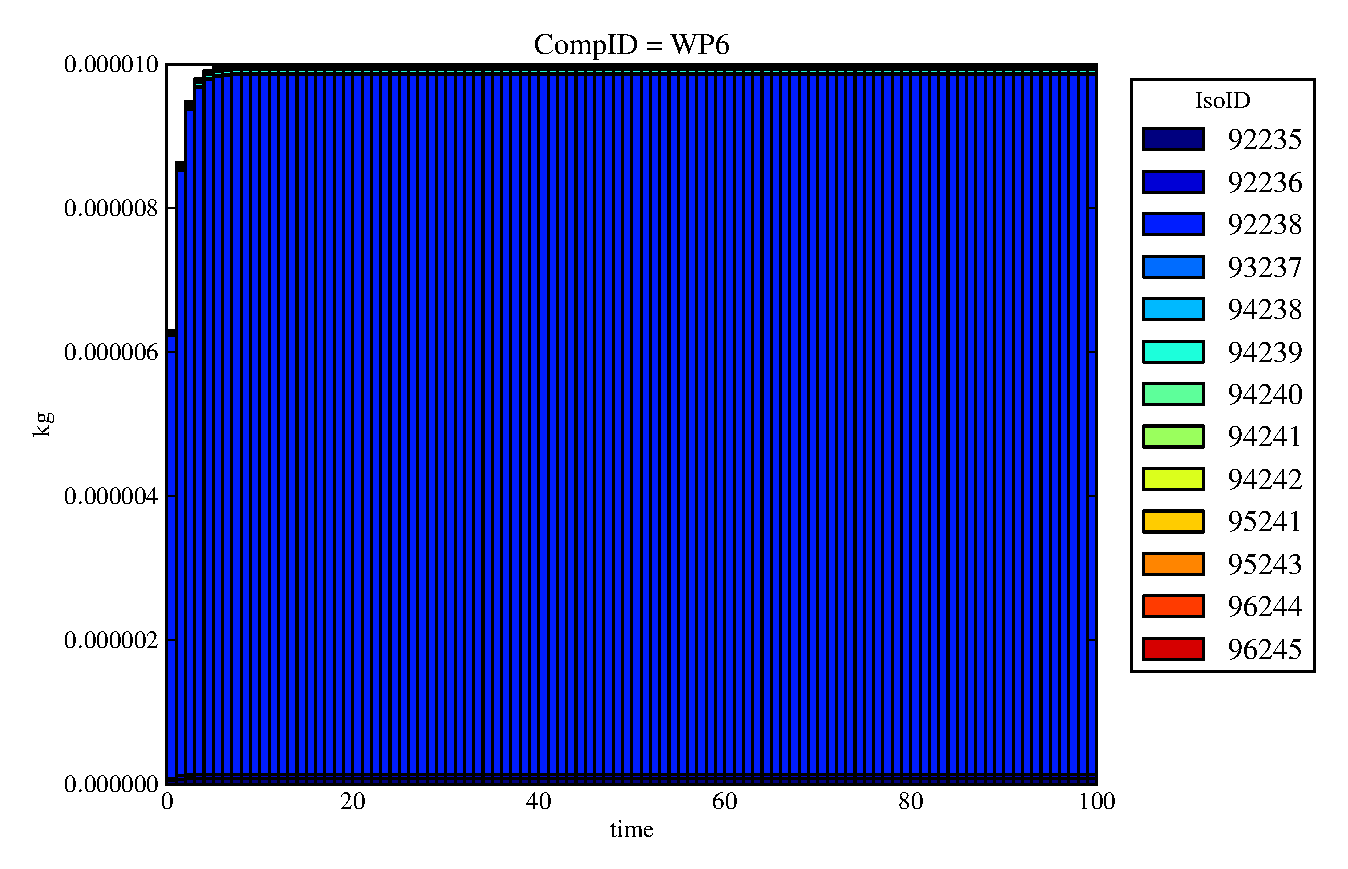
\includegraphics[width=\textwidth]{./chapters/demonstration/base/lpPFMII2.eps}
  \caption[Case LPPFMII Waste Package Contaminants.]{ 
    Waste Package 6 ($F_d = 0.1$) achieves total containment. 
    }
  \label{fig:lpPFMIIwp6}

  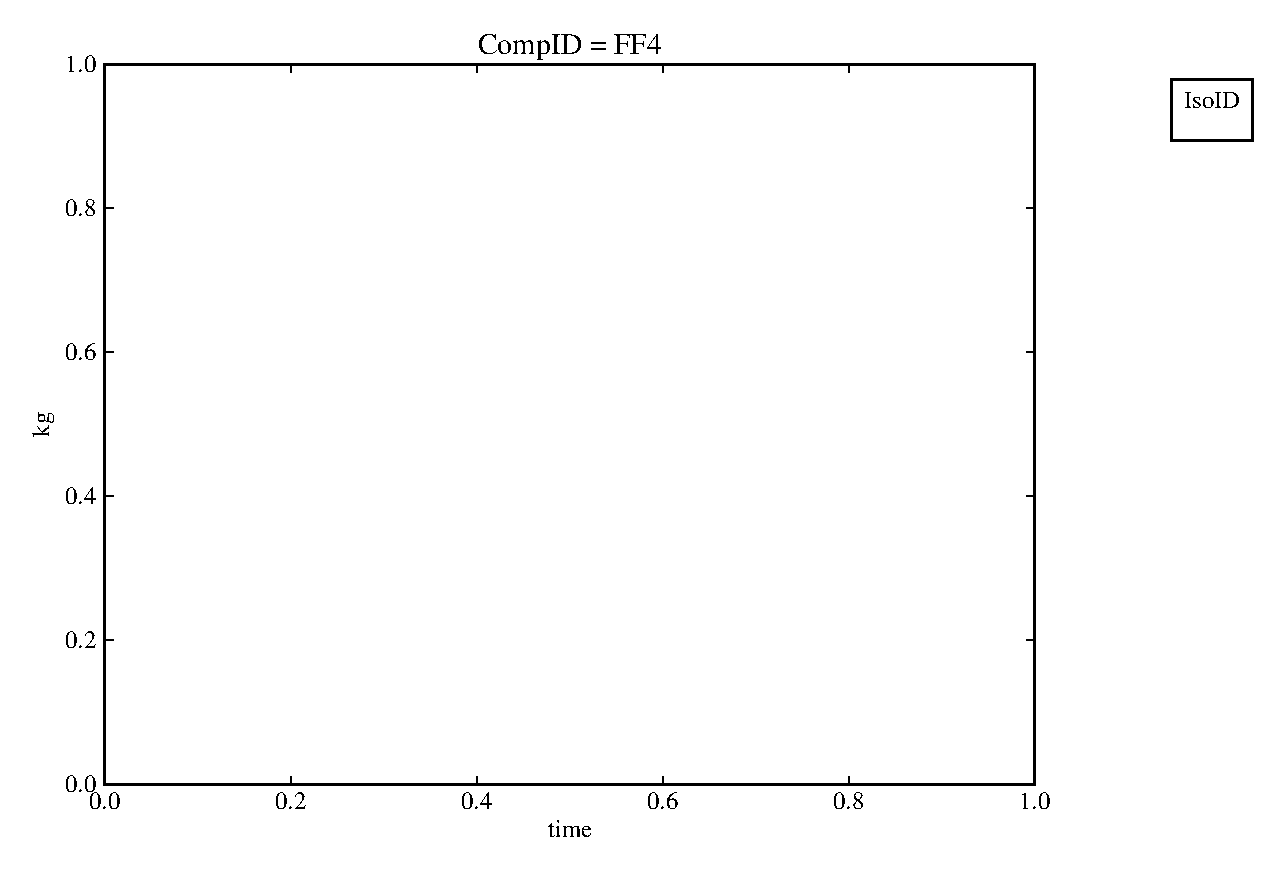
\includegraphics[width=\textwidth]{./chapters/demonstration/base/lpPFMII0.eps}
  \caption[Case LPPFMII Waste Package Contaminants.]{ 
    The Far Field, component 0 ($F_d = 0.1$), never receives material.
    }
  \label{fig:lpEnd}
  \end{minipage}
\end{figure} 

In the second of these simulations, the Exponential Model (EM) was 
selected from among the three response functions. 

\begin{figure}[ht]
\centering
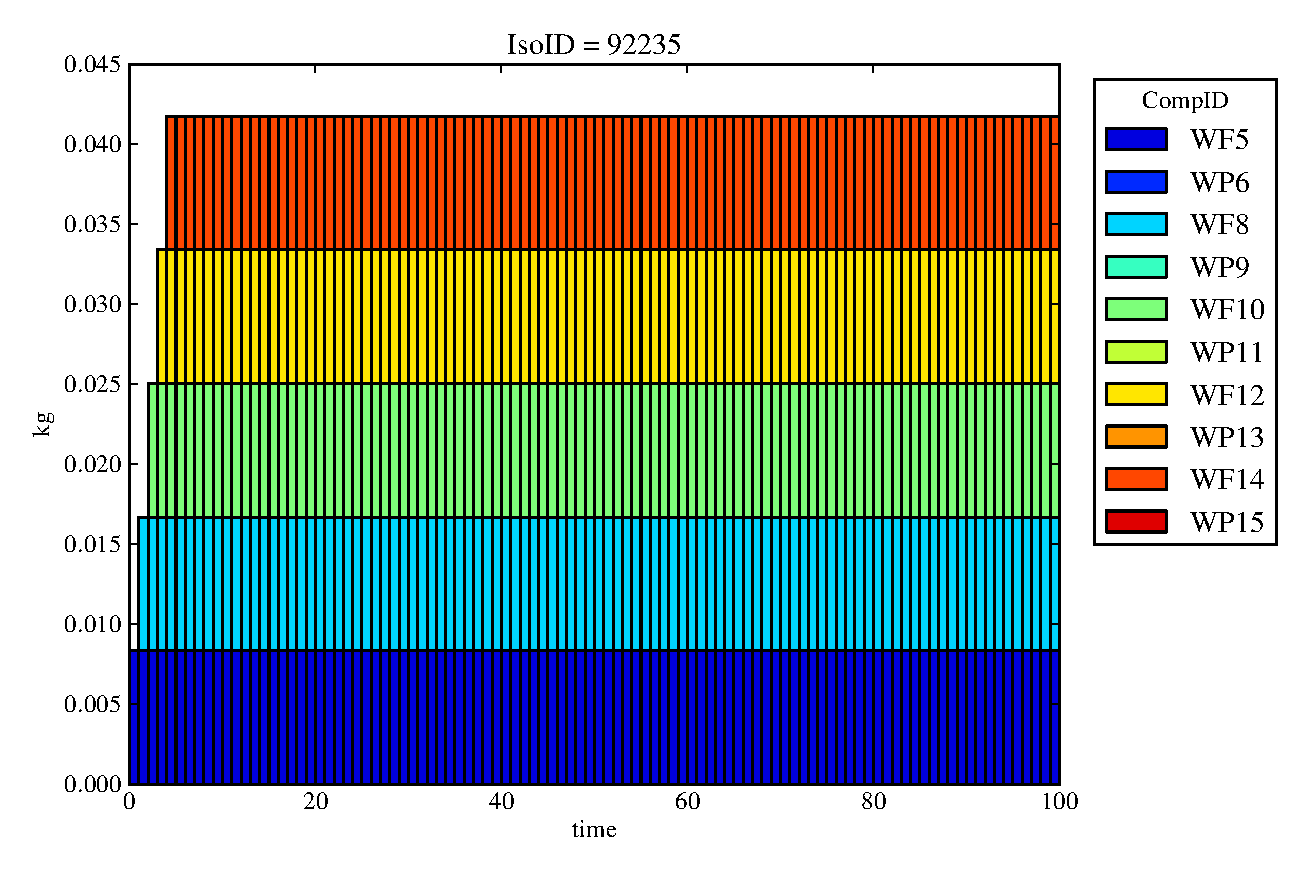
\includegraphics[width=0.6\textwidth]{./chapters/demonstration/base/lpEMII.eps}
\caption[$^{235}U$ residence. Lumped Parameter  Waste Package No Release.]{
For case LPEMII in which total containment in the waste package is assumed 
($F_{d,wp}=0$), $^{235}U$ travels through the waste form component ($F_d = 0.1$) before 
permanent residence in the waste package component.
}
\label{fig:lpBegin}
\begin{minipage}[b]{0.45\linewidth}

  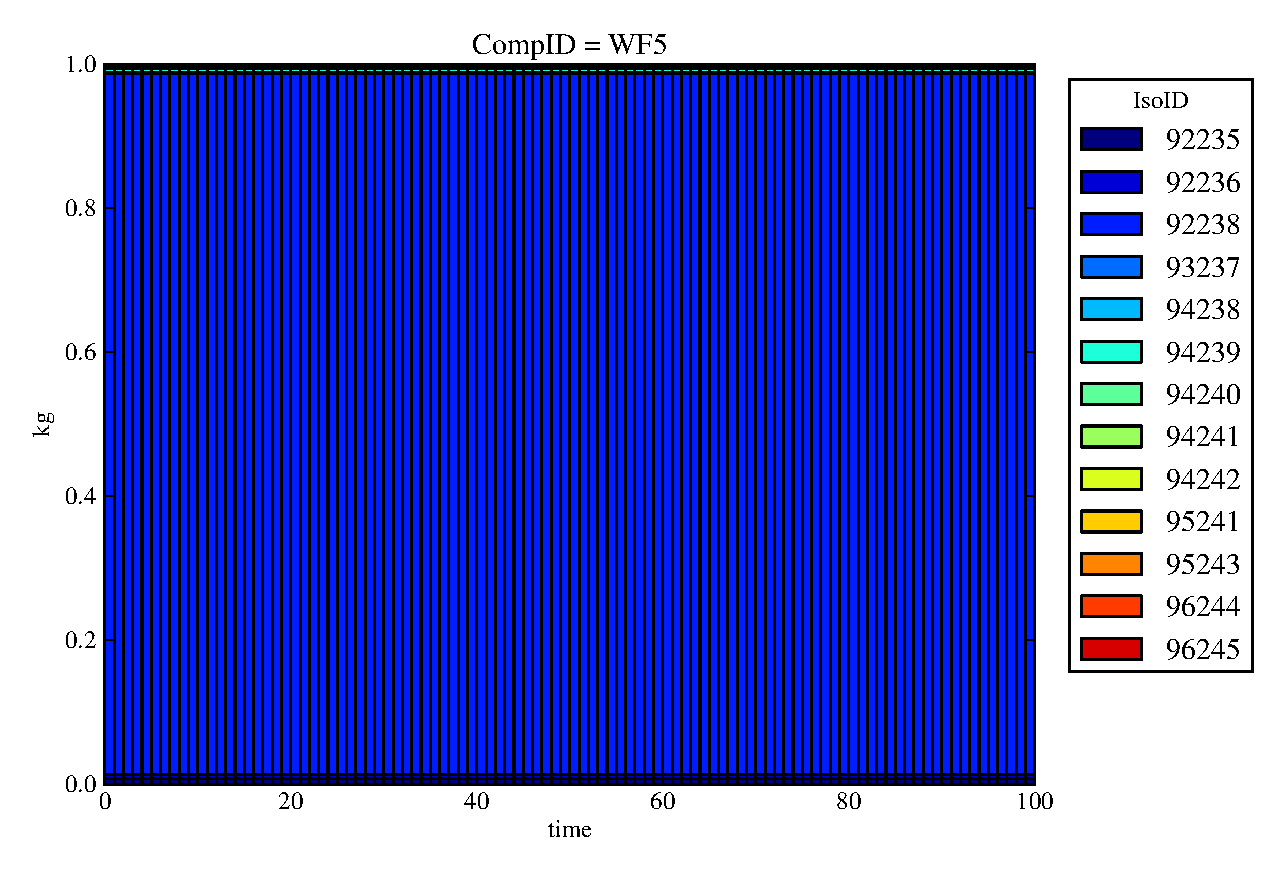
\includegraphics[width=\textwidth]{./chapters/demonstration/base/lpEMII1.eps}
  \caption[Case LPEMII Waste Form Contaminants.]{
    Waste Form 5 ($F_d = 0.1$) releases material with degradation. 
    }
  \label{fig:lpEMIIwf5}
  
  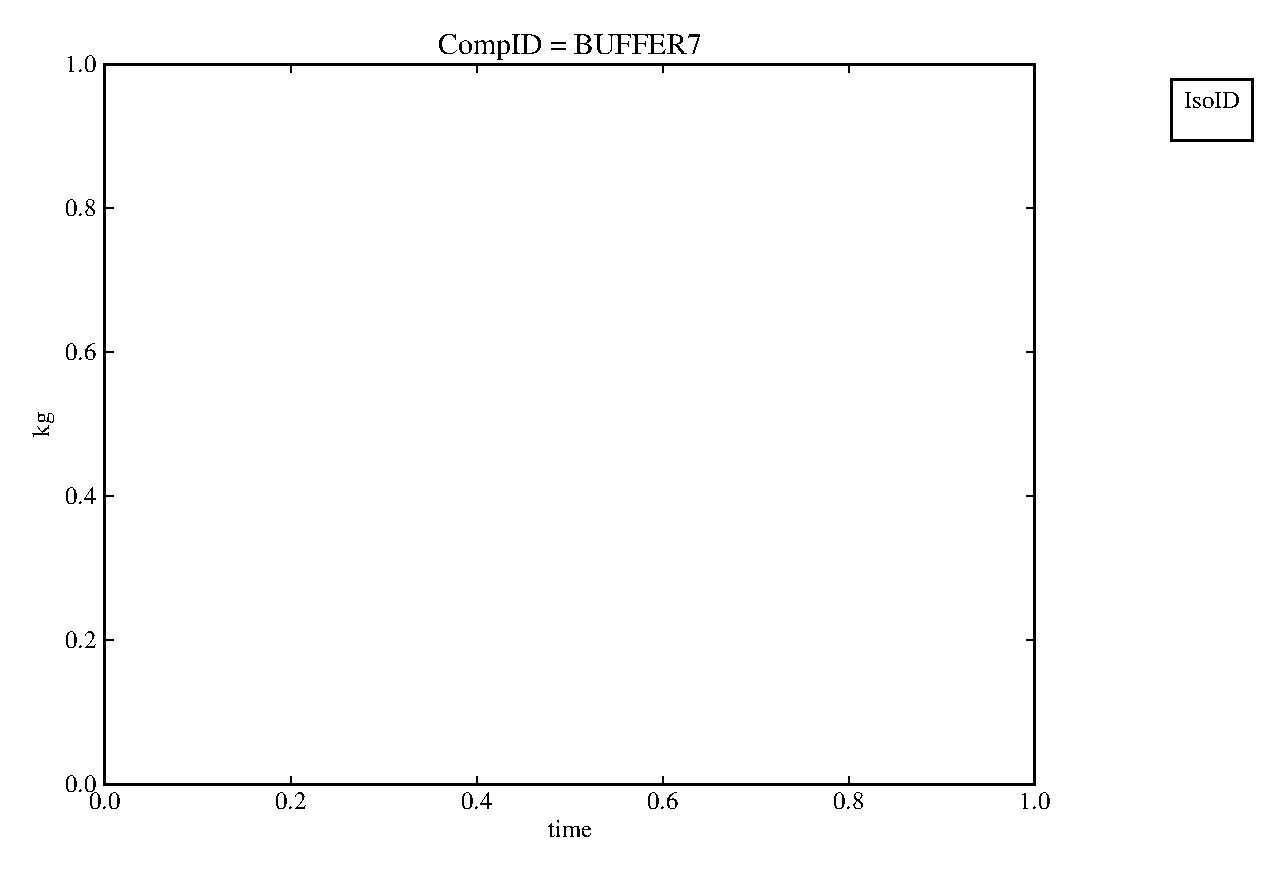
\includegraphics[width=\textwidth]{./chapters/demonstration/base/lpEMII3.eps}
  \caption[Case LPEMII Buffer Contaminants]{
    The Buffer, component 7 ($F_d=0.1$), never receives material.
    }
  \label{fig:lpEMIIbuff}

\end{minipage}
\hspace{0.05\linewidth}
\begin{minipage}[b]{0.45\linewidth}
  \includegraphics[width=\textwidth]{./chapters/demonstration/base/lpEMII2.eps}
  \caption[Case LPEMII Waste Package Contaminants.]{ 
    Waste Package 6 ($F_d = 0.0$) achieves total containment. 
    }
  \label{fig:lpEMIIwp6}

  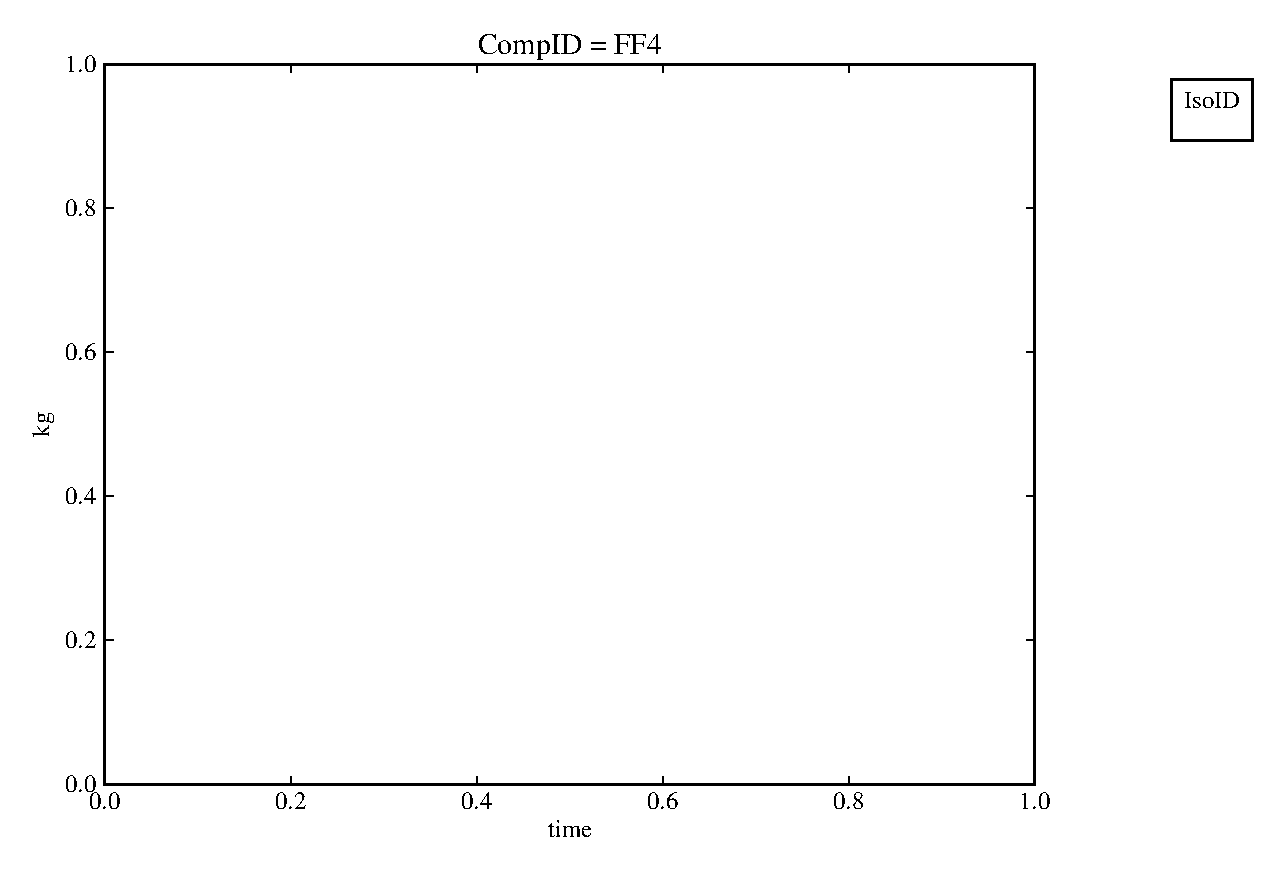
\includegraphics[width=\textwidth]{./chapters/demonstration/base/lpEMII0.eps}
  \caption[Case LPEMII Waste Package Contaminants.]{ 
    The Far Field, component 0 ($F_d = 0.1$), never receives material.
    }
  \label{fig:lpEMIIff0}


  \end{minipage}
\end{figure}

In the second of these simulations, the Dispersion Model (DM) was 
selected from among the three response functions. 

\begin{figure}[ht]
\centering
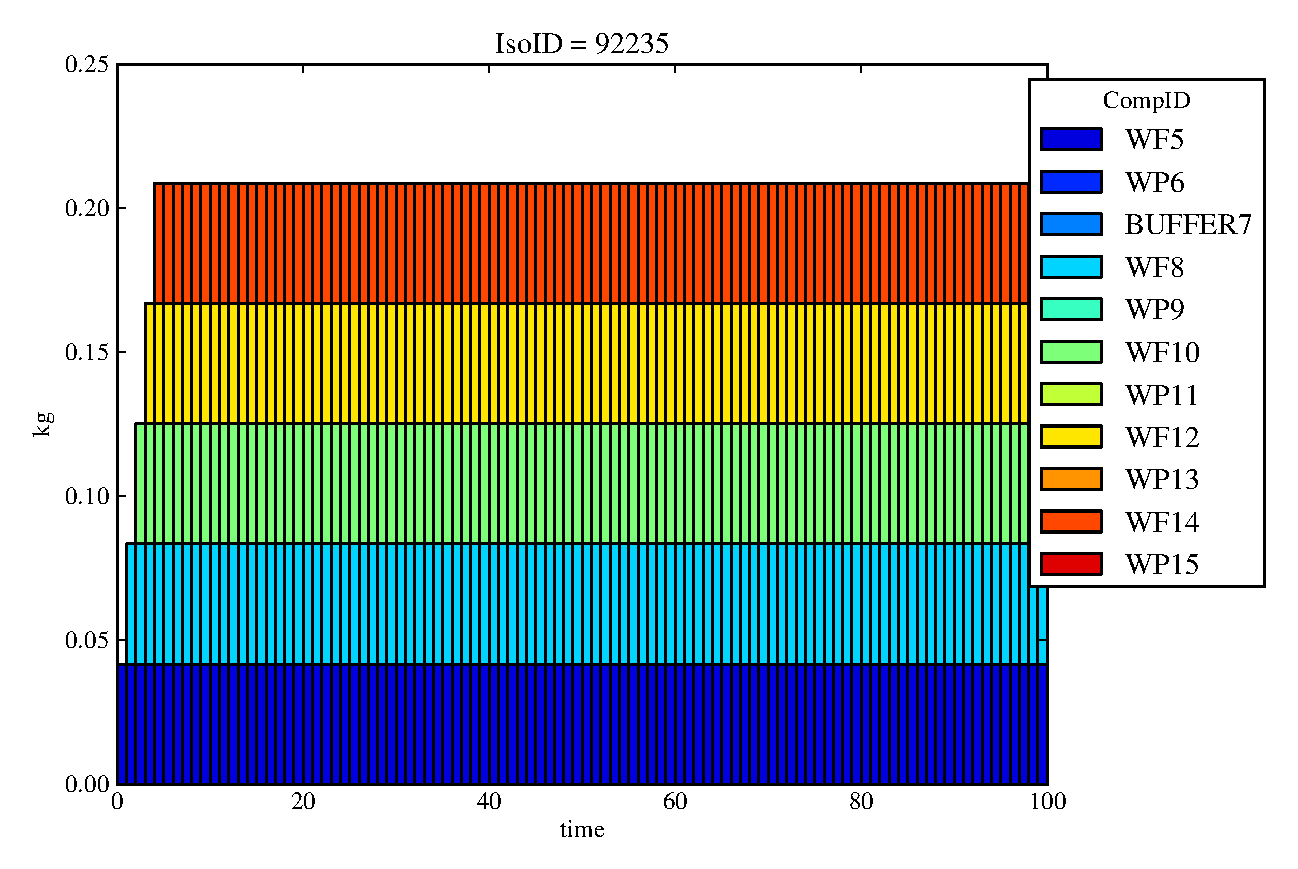
\includegraphics[width=0.6\textwidth]{./chapters/demonstration/base/lpDMII.eps}
\caption[$^{235}U$ residence. Lumped Parameter  DM Waste Package No Release.]{
For LPDMII case in which total containment in the waste package is assumed 
($F_{d,wp}=0$), $^{235}U$ travels through the waste form component ($F_d = 0.1$) before 
permanent residence in the waste package component.
}
\label{fig:lpDMIIall}
\begin{minipage}[b]{0.45\linewidth}

  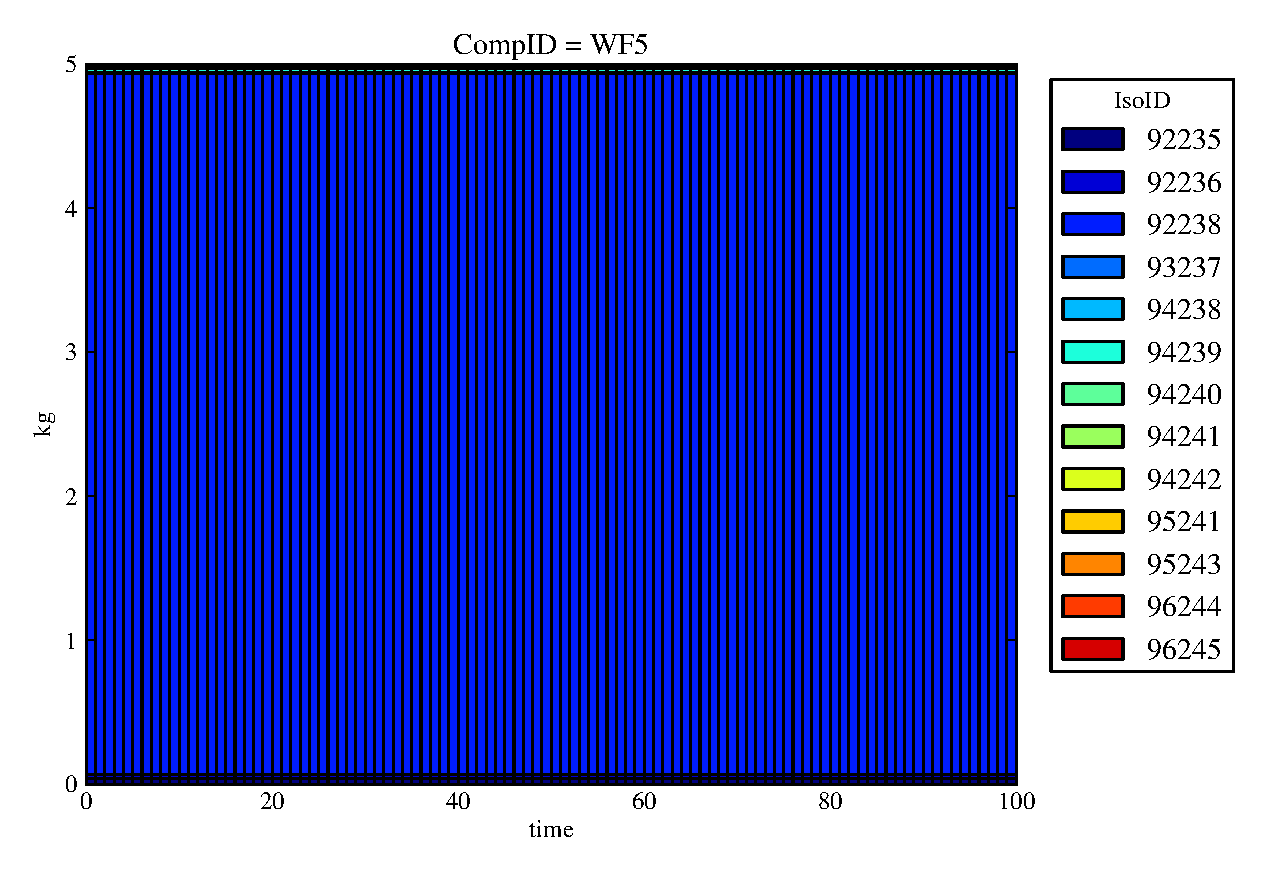
\includegraphics[width=\textwidth]{./chapters/demonstration/base/lpDMII1.eps}
  \caption[Case LPDMII Waste Form Contaminants.]{
    Waste Form 5 ($F_d = 0.1$) releases material with degradation. 
    }
  \label{fig:lpDMIIwf5}
  
  \includegraphics[width=\textwidth]{./chapters/demonstration/base/lpDMII3.eps}
  \caption[Case LPDMII Buffer Contaminants]{
    The Buffer, component 7 ($F_d=0.1$), never receives material.
    }
  \label{fig:lpDMIIbuff}

\end{minipage}
\hspace{0.05\linewidth}
\begin{minipage}[b]{0.45\linewidth}
  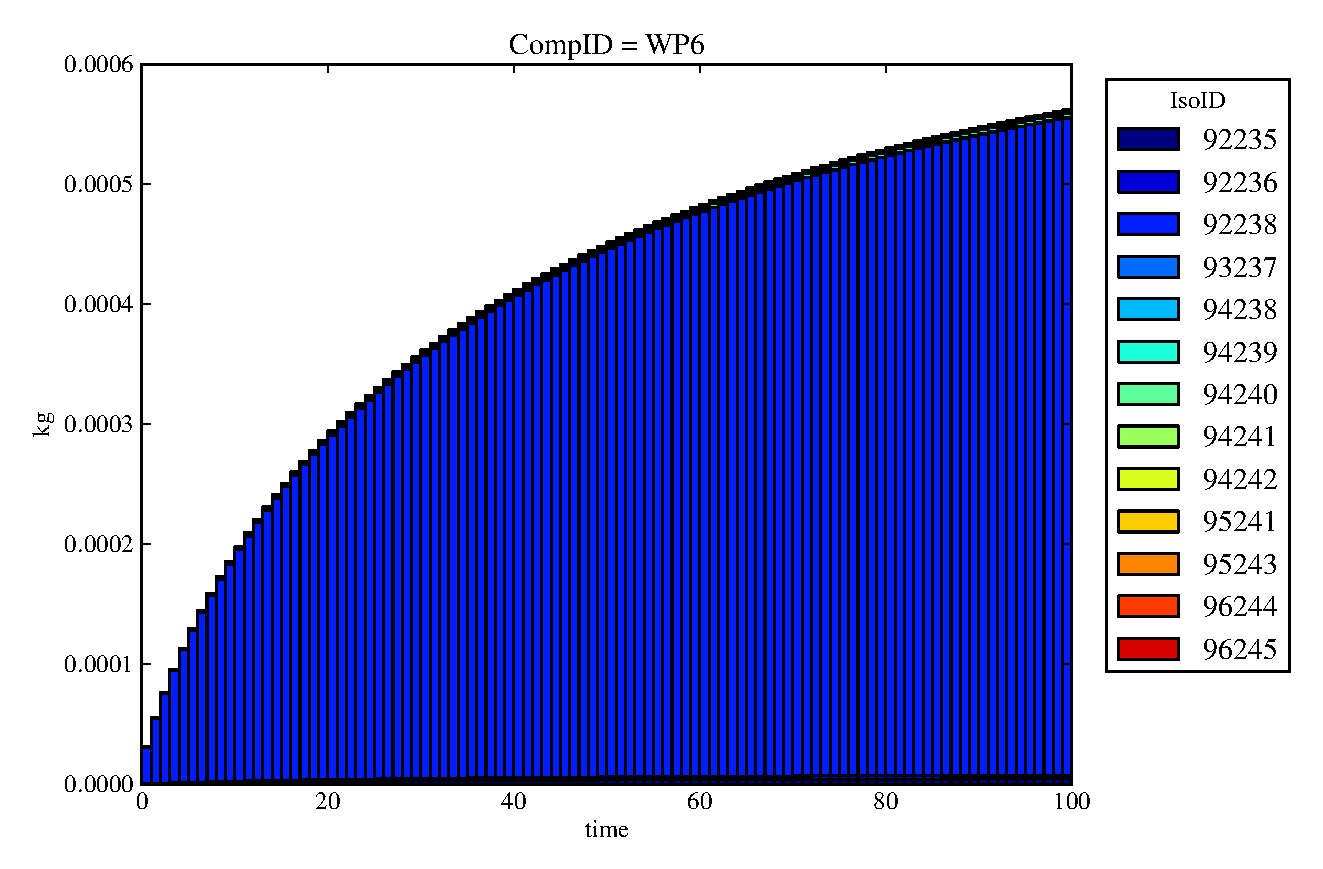
\includegraphics[width=\textwidth]{./chapters/demonstration/base/lpDMII2.eps}
  \caption[Case LPDMII Waste Package Contaminants.]{ 
    Waste Package 6 ($F_d = 0.0$) achieves total containment. 
    }
  \label{fig:lpDMIIwp6}

  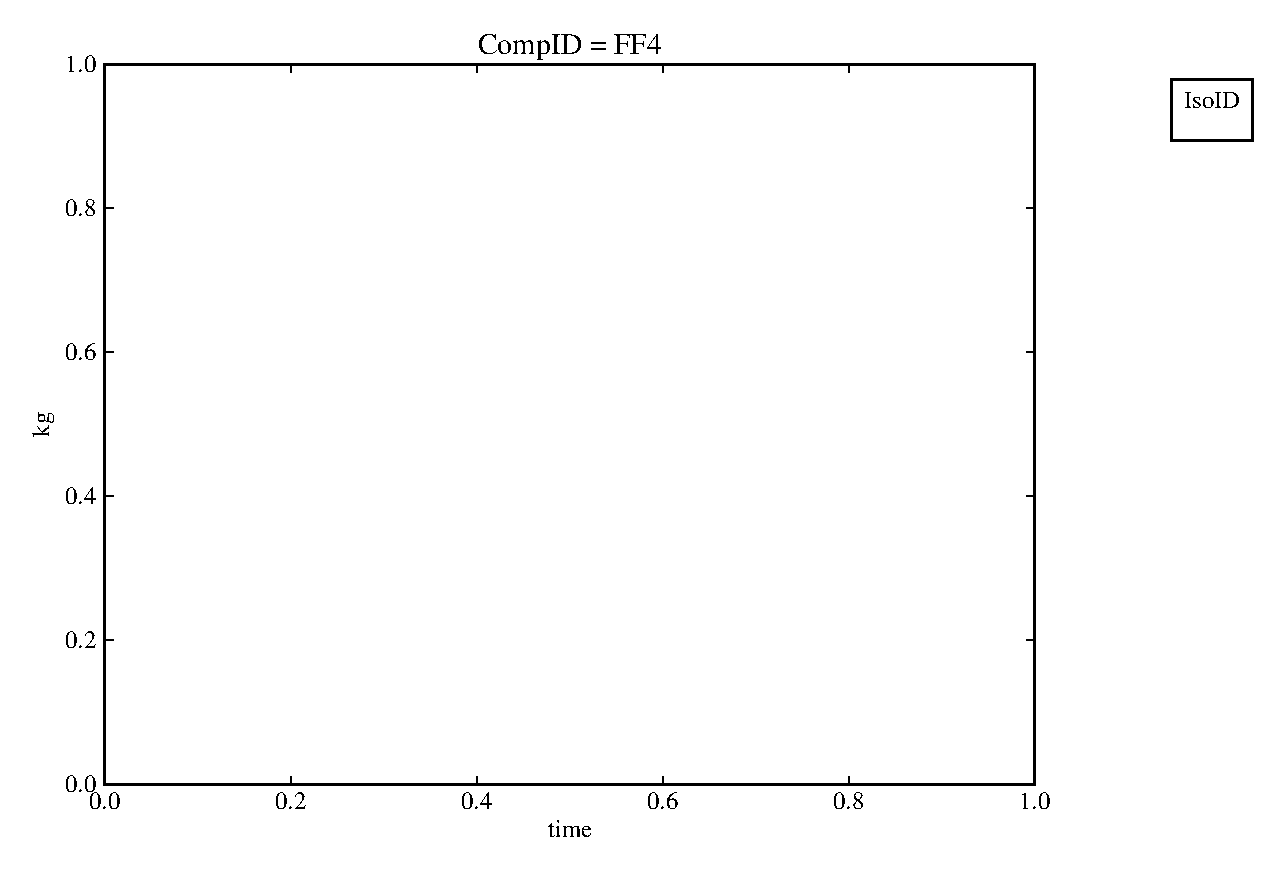
\includegraphics[width=\textwidth]{./chapters/demonstration/base/lpDMII0.eps}
  \caption[Case LPDMII Waste Package Contaminants.]{ 
    The Far Field, component 0 ($F_d = 0.1$), never receives material.
    }
  \label{fig:lpDMIIff0}


  \end{minipage}
\end{figure}

\FloatBarrier
